\chapter{Mengenal Kecerdasan Buatan dan Scikit-Learn}
Buku umum yang digunakan adalah \cite{russell2016artificial} dan  
untuk sebelum UTS menggunakan buku \textit{Python Artificial Intelligence Projects for Beginners}\cite{eckroth2018python}.
Dengan praktek menggunakan python 3 dan editor anaconda dan library python scikit-learn.
Tujuan pembelajaran pada pertemuan pertama antara lain:
\begin{enumerate}
\item
Mengerti definisi kecerdasan buatan, sejarah kecerdasan buatan, perkembangan dan penggunaan di perusahaan
\item
Memahami cara instalasi dan pemakaian sci-kit learn
\item
Memahami cara penggunaan variabel explorer di spyder
\end{enumerate}
Tugas dengan cara dikumpulkan dengan pull request ke github dengan menggunakan latex pada repo yang dibuat oleh asisten riset.

\section{Teori}
Praktek teori penunjang yang dikerjakan :
\begin{enumerate}
\item
Buat Resume Definisi, Sejarah dan perkembangan Kecerdasan Buatan, dengan bahasa yang mudah dipahami dan dimengerti. Buatan sendiri bebas plagiat[hari ke 1](10)
\item
Buat Resume mengenai definisi supervised learning, klasifikasi, regresi dan unsupervised learning. Data set, training set dan testing set.[hari ke 1](10)
\end{enumerate}

\section{Instalasi}
Membuka https://scikit-learn.org/stable/tutorial/basic/tutorial.html. Dengan menggunakan bahasa yang mudah dimengerti dan bebas plagiat. 
Dan wajib skrinsut dari komputer sendiri.
\begin{enumerate}
\item
Instalasi library scikit dari anaconda, mencoba kompilasi dan uji coba ambil contoh kode dan lihat variabel explorer[hari ke 1](10)
\item
Mencoba Loading an example dataset, menjelaskan maksud dari tulisan tersebut dan mengartikan per baris[hari ke 1](10)
\item
Mencoba Learning and predicting, menjelaskan maksud dari tulisan tersebut dan mengartikan per baris[hari ke 2](10)
\item
mencoba Model persistence, menjelaskan maksud dari tulisan tersebut dan mengartikan per baris[hari ke 2](10)
\item 
Mencoba Conventions, menjelaskan maksud dari tulisan tersebut dan mengartikan per baris[hari ke 2](10)
\end{enumerate}


\section{Penanganan Error}
Dari percobaan yang dilakukan di atas, apabila mendapatkan error maka:

\begin{enumerate}
	\item
	skrinsut error[hari ke 2](10)
	\item
Tuliskan kode eror dan jenis errornya [hari ke 2](10)
	\item
Solusi pemecahan masalah error tersebut[hari ke 2](10)

\end{enumerate}

\section{Teori}
Teori mencakup resume dari beberapa pembahasan. yaitu :
\begin{enumerate}
\begin
\item Definisi Kecerdasan Buatan.
\par Jadi yang dimaksud dengan  kecerdasan buatan yaitu  salah satu dari cabang Ilmu pengetahuan yang kita punya dan  berhubungan juga dengan pemanfaatan mesin yaitu untuk dapat memecahkan suatu  persoalan yang rumit dengan  menggunakan cara yang lebih manusiawi.
\par Jadi yang dimaksud dengan supervised learning  adalah pembelajaran mesin yang diawasi menciptakan model yang melancarkan prediksi berdasarkan bukti adanya ketidakpastian. Algoritma pembelajaran yang diawasi memerlukan seperangkat data masukan dan tanggapan yang diketahui terhadap data (output) dan melatih model untuk menghasilkan prediksi yang masuk akal untuk respon terhadap data baru. Sedangkan untuk klasifikasi yaitu nilai output yang  bernilai diskrit (kelas) dan Bertujuan mengklasifikasi data baru dengan akurat diawasi dengan menggunakan teknik klasifikasi dan regresi untuk mengembangkan model prediktif. Yang dimaksud dengan regresi adlah nilai output yang bernilai kontinu (riil), Bertujuan memprediksi output dengan akurat untuk data baru.
\par Unsupervised learning tidak menggunakan data latih atau data training untuk melakukan prediksi maupun klasifikasi. Berdasarkan model matematisnya, algoritma ini tidak memiliki target variabel. Salah satu tujuan dari algoritma ini adalah mengelompokkan objek yang hampir sama dalam suatu area tertentu. Dan yang dimaksud dengan  Dataset adalah objek yang merepresentasikan data dan relasinya di memory. Strukturnya mirip dengan data di database. Dataset berisi koleksi dari datatable dan datarelation. Sedangkan testing set digunakan untuk mengukur sejauh mana classifier berhasil melakukan klasifikasi dengan benar. Dan training set digunakan oleh algoritma klassifikasi untuk membentuk sebuah model classifier. Model yang dimaksud ini merupakan representasi pengetahuan yang akan digunakan untuk prediksi kelas data baru yang belum pernah ada.
\end{enumerate} 

\section
\item 
Mencoba Learning and predicting, menjelaskan maksud dari tulisan tersebut dan mengartikan per baris[hari ke 2](10)
\begin{figure}
	\begin{center}
   	 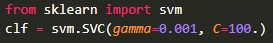
\includegraphics[scale=0.5]{figures/cahya1.png}
   	 \caption{capturing}	
	\end{center}
\end{figure}
Pada gambar diatas dapat dijelaskan bahwa :\\
Baris yang pertama  kita memasukkan dan memanggil svm dari sklearn.\\
Baris yang kedua  kita membuat variable.\\
\item)
\begin{figure}
	\begin{center}
   	 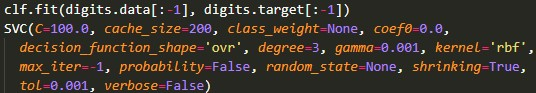
\includegraphics[scale=0.5]{figures/cahya2.png}
   	 \caption{capturing}	
	\end{center}
\end{figure}
Pada gambar diatas dapat dijelaskan bahwa :\\
Baris yang pertama itu clf dipasang pada model fit metode.\\
Baris yang kedua kita implementasikan klasifikasi dukungan vektor.\\
\item 
\begin{figure}
	\begin{center}
   	 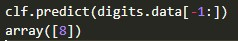
\includegraphics[scale=0.5]{figures/cahya3.png}
   	 \caption{capturing}	
	\end{center}
\end{figure}
Pada gambar diatas dapat dijelaskan bahwa :\\
Baris yang pertama itu untuk prediksi nilai baru.\\
Baris yang kedua untuk set array.\\

\end{enumerate}

\section
\item 
mencoba Model persistence, menjelaskan maksud dari tulisan tersebut dan mengartikan per baris[hari ke 2](10)
\begin{figure}
	\begin{center}
   	 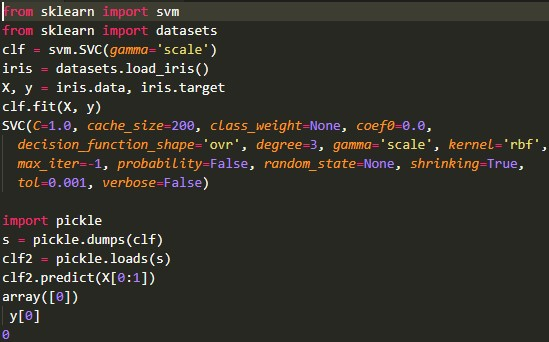
\includegraphics[scale=0.5]{figures/cahya4.png}
   	 \caption{capturing}	
	\end{center}
\end{figure}
Pada gambar diatas dapat dijelaskan bahwa :\\
Baris yang pertama kita memasukkan dan memanggil datasets dari sklearn.\\
Baris yang kedua kita memasukkan dan memanggil svm dari sklearn.\\
Baris yang ketiga kita  membuat variable clf.\\
Baris yang keempat kita  membuat variable iris.\\
Baris yang kelima kita  membuat variable x, y.\\
Baris yang keenam  clf dipasang pada model fit metode.\\
Baris yang ke tujuh kita  implementasikan klasifikasi dukungan vektor.\\
Baris yang kedelapan kita memanggil library pickle.\\
Baris yang kesembilan untuk  membuat variable s.\\
Baris yang kesepuluh untuk  membuat variable clf2.\\
Baris yang keseblas untuk  prediksi nilai baru.\\
Baris yang keduabelas untuk  set array.\\

\end{enumerate}


\item 
Mencoba Conventions, menjelaskan maksud dari tulisan tersebut dan mengartikan per baris[hari ke 2](10)
\begin{figure}
	\begin{center}
   	 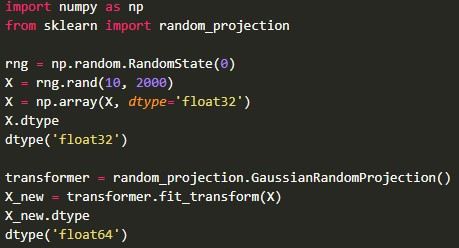
\includegraphics[scale=0.5]{figures/cahya5.png}
   	 \caption{capturing}	
	\end{center}
\end{figure}
Pada gambar diatas dapat dijelaskan bahwa :\\
Baris yang pertama kita memasukkan dan memanggil numpy sebagai np.\\
Baris yang kedua kita memasukkan dan memanggil random_projection dari sklearn.\\
Baris yang ketiga kita  membuat variable rng.\\
Baris yang keempat untuk  membuat variable rng.\\
Baris yang kelima untuk  membuat variable x.\\
Baris yang keenam untuk  pemanggilan variable x.\\
Baris yang ketujuh untuk pemanggilan dtype.\\
Baris yang kedelapan kita membuat variable tranformer.\\
Baris yang kesembilan kita membuat variable x_new.\\
Baris yang kesempulah untuk  pemanggilan x_new.\\
Baris yang keseblas untuk  pemanggilan dtype.\\

\end{enumerate}